% Chris Hodapp, 2016-04-25
% Georgia Institute of Technology, CS6475, Computational Photography,
% Spring 2016
% Final Project

\documentclass{article}
\usepackage{amsmath}
\usepackage{graphicx}
\usepackage{float}
\usepackage{hyperref}
\usepackage[letterpaper, portrait, margin=1in]{geometry}

\title
    {CS6475, Computational Photography \\
      Spring 2016 \\
      Final Project}
\date{April 25, 2016}
\author{Chris Hodapp, chodapp3@gatech.edu}

\begin{document}
\maketitle

\section{Literate Implementation of ``A Neural Algorithm of Artistic Style''}

\subsection{Project Goal}

The goal of this project was to create a literate implementation (as
in \href{https://en.wikipedia.org/wiki/Literate_programming}{literate
  programming}) of the algorithm described in the recent paper, ``A
Neural Algorithm of Artistic Style'' by Leon A. Gatys, Alexander
S. Ecker, and Matthias Bethge\cite{neuralstyle2015}.

The paper is sufficiently well-known by now that it has many
open-source and commercial implementations that are quite good:

\begin{itemize}
  \item \url{https://github.com/jcjohnson/neural-style}
  \item \url{https://github.com/kaishengtai/neuralart}
  \item \url{https://github.com/andersbll/neural_artistic_style}
  \item \url{https://github.com/fzliu/style-transfer}
  \item \url{https://github.com/woodrush/neural-art-tf}
  \item \url{https://deepart.io}
\end{itemize}

However, I found that many of these lacked clear explanations on why
they were implemented how they were.

The students in this class (and others such as CS6476) should already
be familiar to some degree with the use of Python, NumPy, SciPy, and
OpenCV in the algorithms of computational photography.  My aim was
that this implementation let such students use this familiarity as a
stepping stone to understanding the clever methods in this paper and
libraries like the \href{http://caffe.berkeleyvision.org/}{Caffe} deep
learning framework.

The eventual result was an IPython notebook (via
\href{https://jupyter.org/}{Jupyter}) which gives a simplified (but
still functional) example of how to actually implement this algorithm.
All images in this report were produced with that code.

\subsection{Credits \& Acknowledgements}

The implementation here derives from all of the open-source projects
listed above along with the aforementioned research
paper\cite{neuralstyle2015}.  The particular Python approach was based
on \href{https://github.com/fzliu/style-transfer}{style-transfer} by
Frank Lie and Dylan Paiton, and some techniques came from
\href{https://github.com/jcjohnson/neural-style}{neural-style} from
Justin Johnson.

It also makes extensive use of the
\href{http://caffe.berkeleyvision.org/}{Caffe} deep learning framework
and the BVLC Reference CaffeNet from the
\href{http://caffe.berkeleyvision.org/model_zoo.html}{Caffe Model
  Zoo}.

\subsection{Resources}

This file contains the Python notebook:

\url{http://hodapple.com/files/cs6475/chodapp3-cs6475-neural-style.zip}.

This presently requires Python 2.x with NumPy, SciPy, OpenCV, and
\href{http://caffe.berkeleyvision.org/}{Caffe}.  Presently, the only
reason for not supporting Python 3.x is that the Caffe bindings only
support Python 2.x.

Running this will require a pre-trained Caffe model such as one from
the \href{http://caffe.berkeleyvision.org/model_zoo.html}{Caffe Model
  Zoo}.  As the model used here is 200+ MB, it is left out of the ZIP
file above.  The code notes where to download this model and how to
swap it out for different models if desired.

Using the notebook requires an installation of
\href{https://jupyter.org/}{Jupyter} and IPython.  Merely viewing the
notebook can be done without needing dependencies listed above,
however, to actually run the code of course requires those
dependencies.

The file also contains Python code exported from the notebook.  It may
require that a handful of lines using \texttt{IPython.display} be
removed, but they are there only for visualization in the notebook.

An exported version of this notebook also appears later on in this
report.

\subsection{Pipeline}

The below shows a rough pipeline for how this algorithm operates.  The
inputs are the style image and output images, and the output is the
generated image.  The neural network, loss function, and optimization
process have many parameters influencing the result, but they are not
shown here.

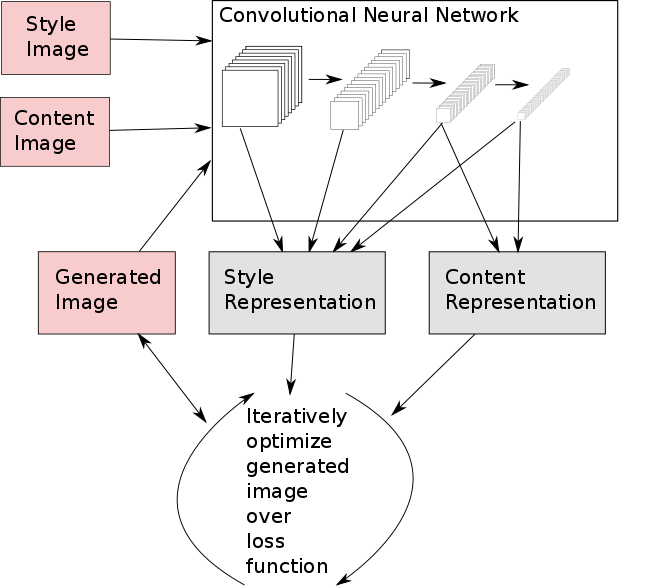
\includegraphics[width=0.7\textwidth]{flowchart.png}

Much more detail is available in the Python notebook that is attached
at the end of this document, as well as the research paper that is
referenced.

\subsection{Images}

Getting images that looked right with this code took a lot of
experimentation. Two examples are given below (the first of which is
also reproduced in the Python notebook that is attached).

\subsubsection{Great Wave \& French Park}

The style image used for this example was the well-known illustration,
\href{https://en.wikipedia.org/wiki/The_Great_Wave_off_Kanagawa}{The
  Great Wave off Kanagawa}:

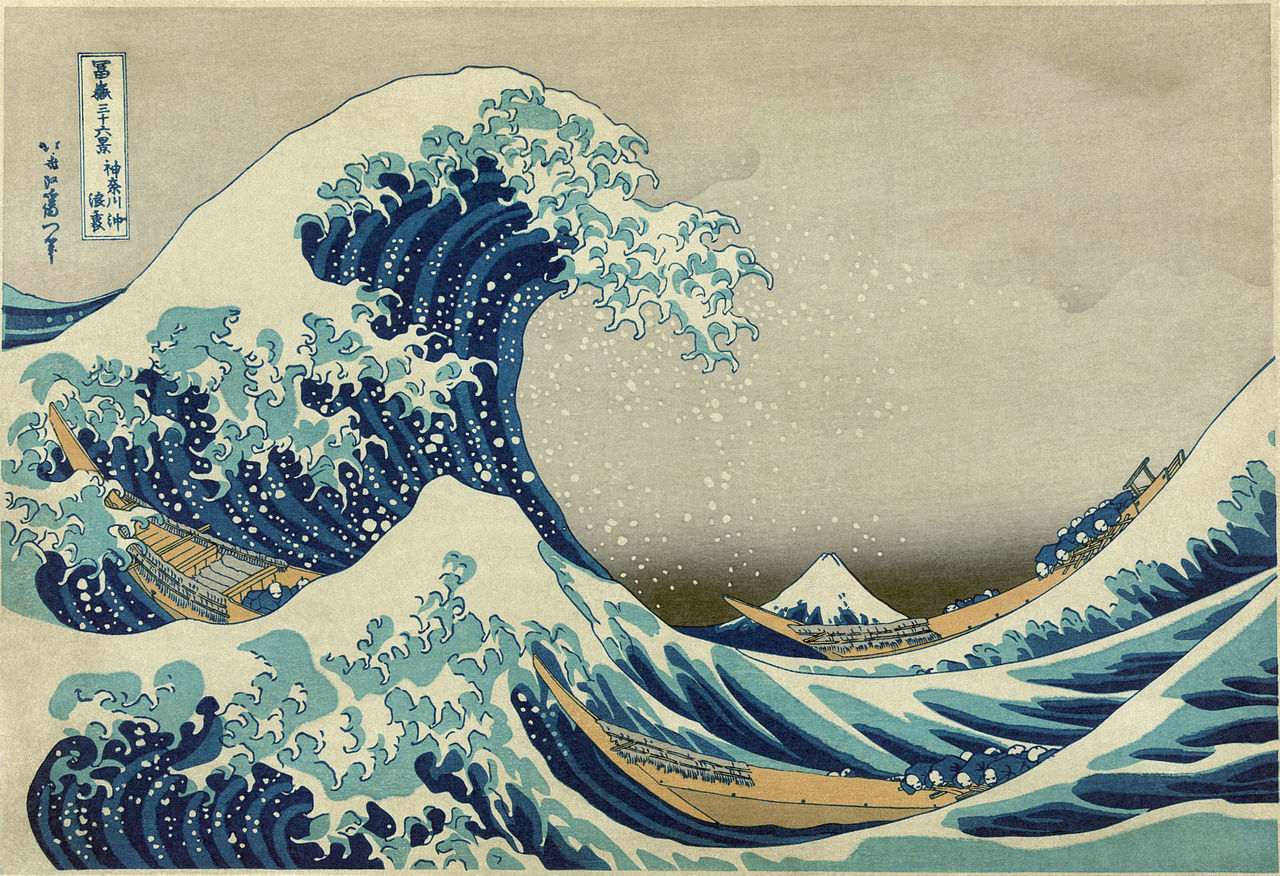
\includegraphics[width=0.7\textwidth]{./1280px-Great_Wave_off_Kanagawa2b.jpg}

The content image is a photograph taken on my phone on Section
Rd. near French Park in Cincinnati, Ohio:

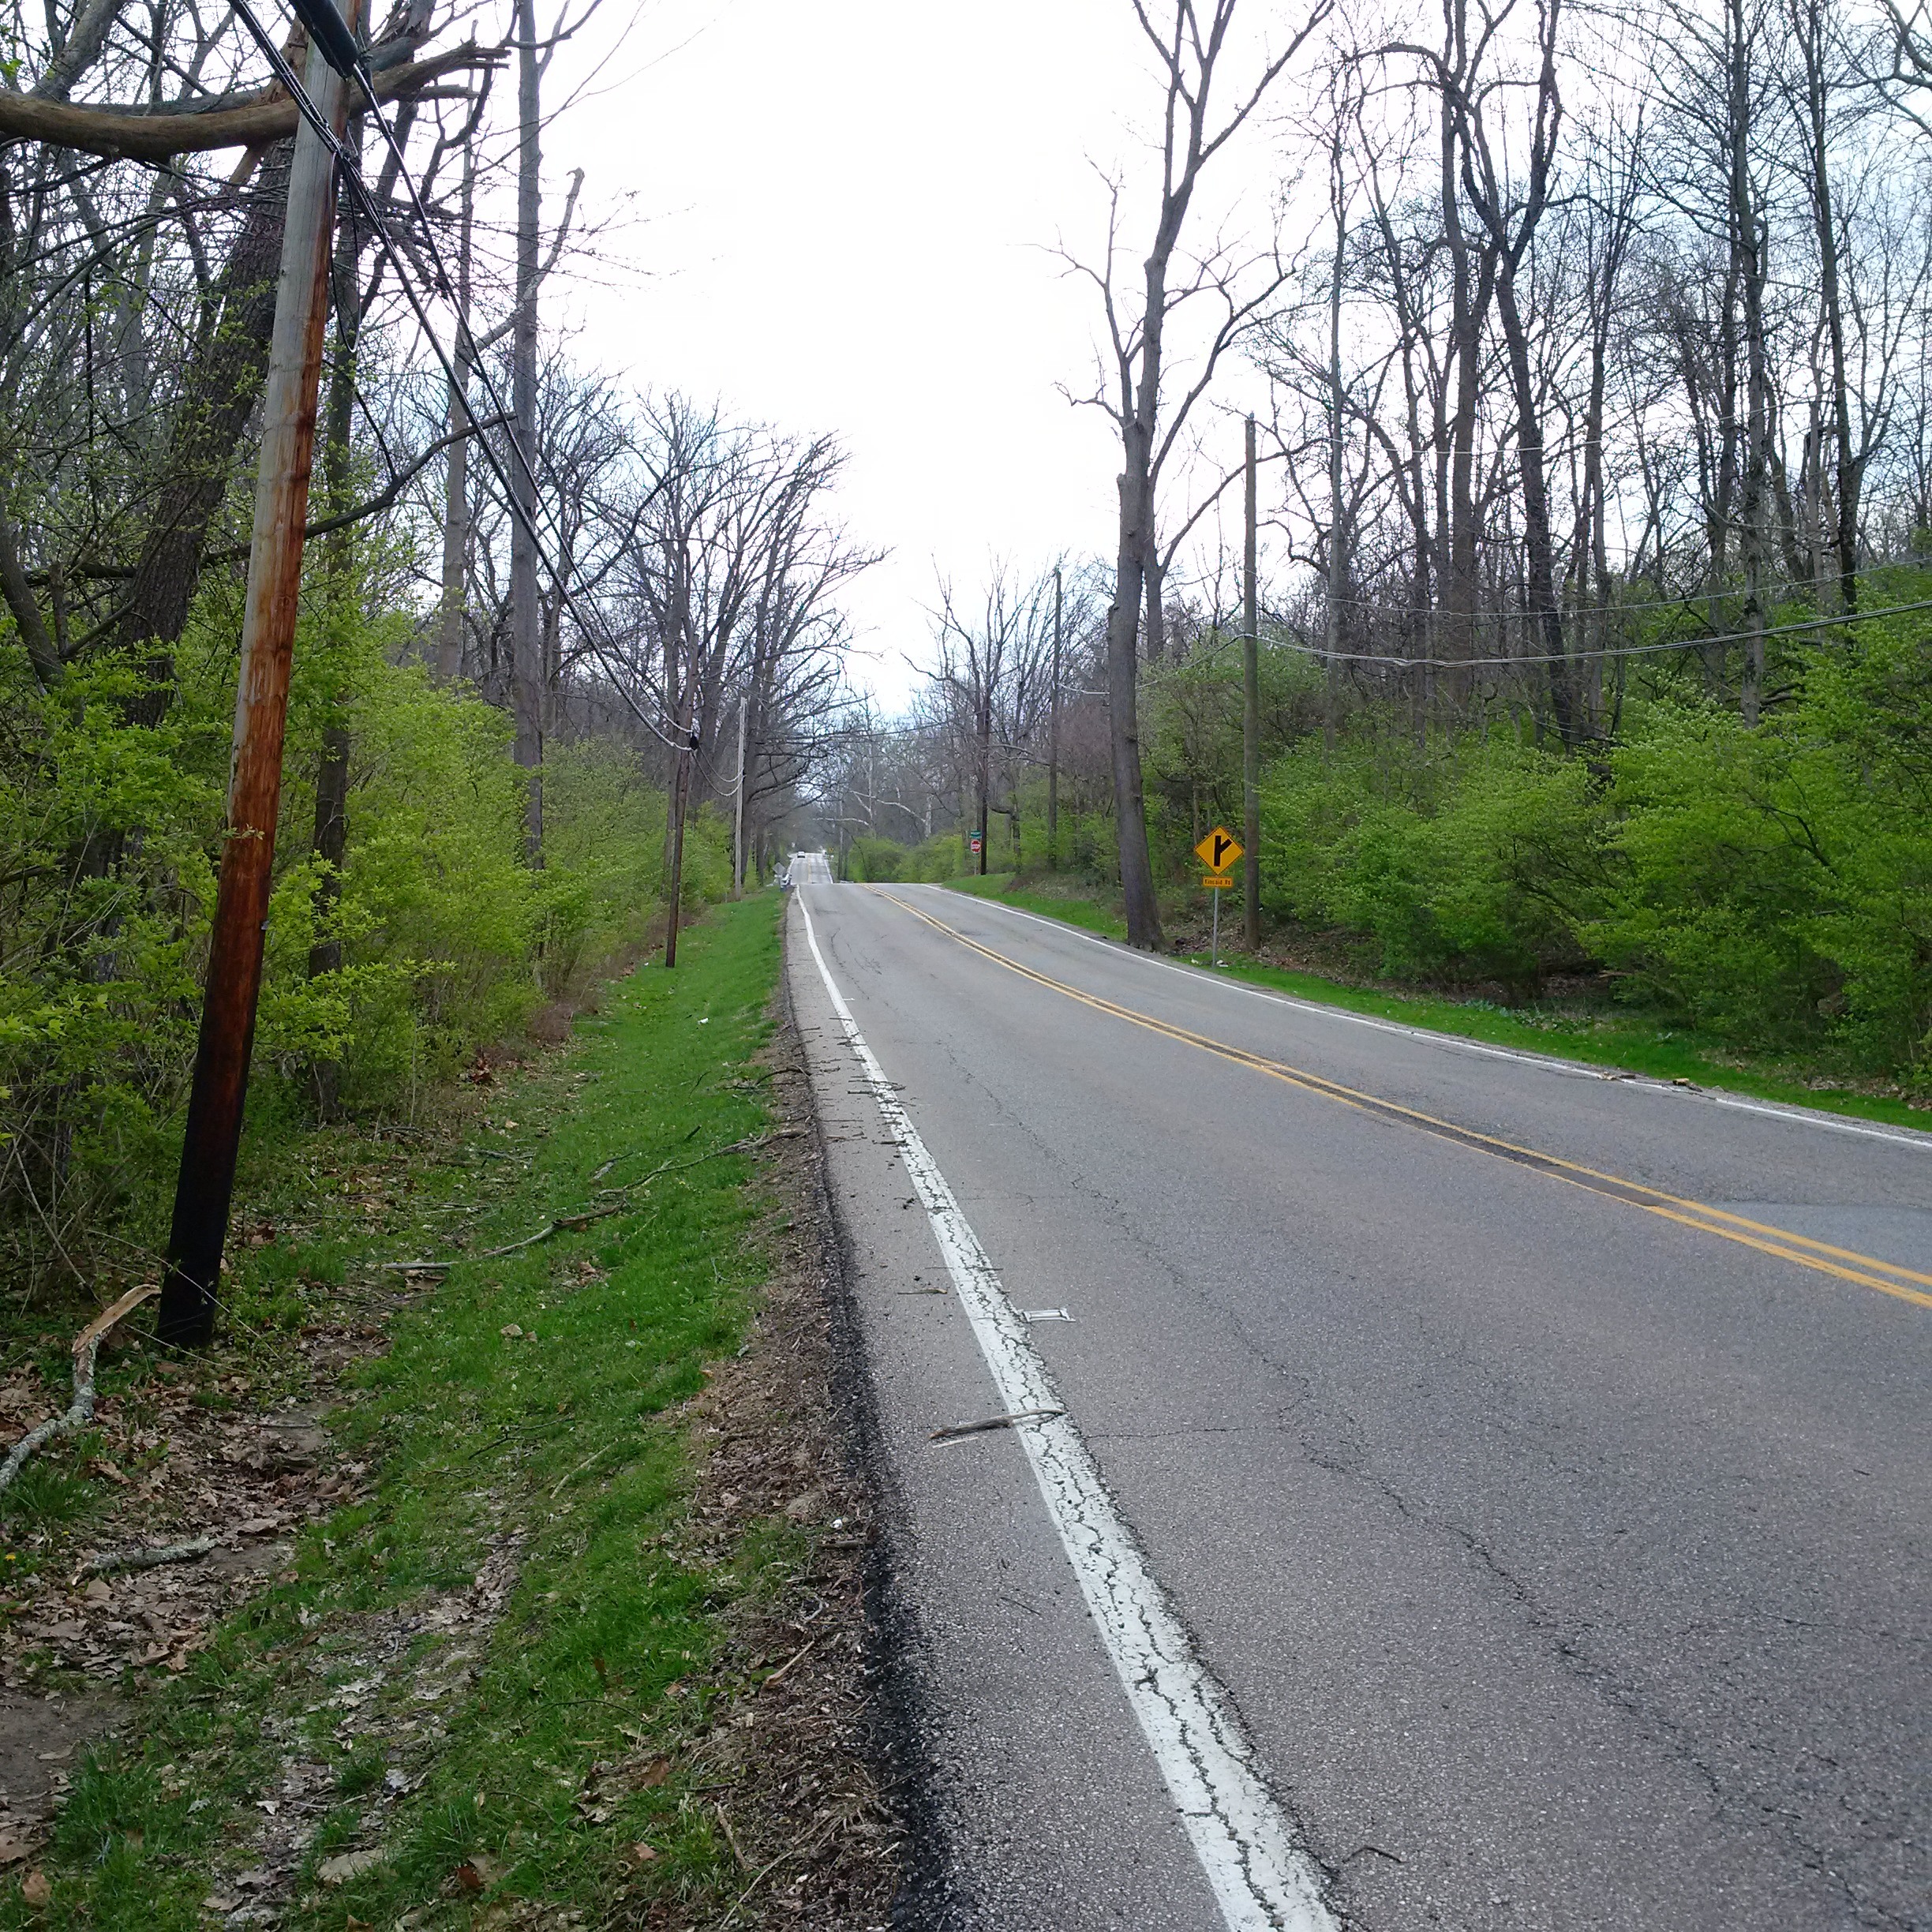
\includegraphics[width=0.7\textwidth]{./french_park.jpg}

Finally, the below is the result of running the given code in order to match the
style of the first image with the content of the second.
Particularly, it is a 1024x1024 image, it used layers \texttt{conv1},
\texttt{conv2}, \texttt{conv3}, \texttt{conv4}, and \texttt{conv5} of
the neural network for the style representation, and \texttt{conv4}
for the content representation, and it ran for 400 iterations with
$\alpha=1$, $\beta=10^3$, and $TV=10^-2$.

\includegraphics[width=0.9\textwidth]{./out_french_c4_all.jpg}

Many more parameters exist that could be tuned, and I make no attempt
to show them all, but the grid below shows different combinations of
layers being used for the style and the content representations:

\includegraphics[width=1.00\textwidth]{./frenchpark_composite.jpg}

\subsubsection{Autumn illustration \& Harrisburg}

The style image is an illustration from Jessica Lanan titled
\href{http://jessicalanan.com/an-autumn-stroll/}{An Autumn Stroll}:

\includegraphics[width=0.7\textwidth]{./Fall-FB.jpg}

The content image is a photograph from Harrisburg, Pennsylvania:

\includegraphics[width=0.7\textwidth]{./harrisburg.jpg}

The result is the 1280x960 image below, rendered with near-identical
settings as the last example (except for $\beta=10^4$ - i.e. putting
more focus on the style):

\includegraphics[width=0.9\textwidth]{./out_harrisburg.jpg}

\subsection{What Worked \& What Didn't}

This algorithm required a lot of tuning to get results that were
appealing, and the attached notebook may give some sense of how many
parameters it has that could require tuning.  The fact that the
results were subject to some amount of randomness and that the
parameters seemed scale-dependent also made tuning difficult.  On the
other hand, the algorithm did seem to provide a lot of control.

It seemed very sensitive to textures, and it had problems with
photographs that were higher-detail; this was not so much an issue of
the photograph's resolution as it was the presence of fine edges.

It seemed as though the style image needed to have a sufficient range
of color and texture in it in order to be able to represent the
content well.  Poor settings or unsuitable style images seemed to
manifest themselves as the content image being completely
unrecognizable, or as the content image being visible as a mosaic of
the same pieces of the style image over and over.

I quickly ran into the memory and processing limits.  My video card
was an Nvidia GTX 660 Ti with 2 GB of memory, and while some neural
networks fit in this memory, many others (the preferred ones) could
not.  In addition, it put a limit on how large of an image I could
generate.  While I could have run all of these operations on my CPU,
this would have taken between hours and days for a single image.

All my tests were run with a pre-trained Caffenet neural network.  I
witnessed better results on a GoogleNet neural network, but with
longer processing time.  I wanted to test further on other neural
networks, particularly with the Illustration2Vec network that was
designed and trained on illustrations\cite{Saito2015}, but my video
card had insufficient memory for these networks.

I still feel I was able to get good results using content images from
photographs that had recognizable overall scenes, and style images
from illustrations that covered a similar range of colors.

\begin{thebibliography}{9}

\bibitem{neuralstyle2015} Leon A. Gatys, Alexander S. Ecker, and
  Matthias Bethge, A Neural Algorithm of Artistic Style,
  \emph{arXiv:1508.06576v2}, \url{http://arxiv.org/abs/1508.06576},
  2015.

\bibitem{Saito2015}Masaki Sati and Yusuke Matsui,
  Illustration2Vec: A Semantic Vector Representation of Illustrations,
  \emph{SIGGRAPH Asia Technical Briefs}, 2015.
  
\end{thebibliography}

\section{Python notebook}

What follows after this is an exported version of the Python notebook
that is linked earlier.

\end{document}
